\documentclass{article}
\usepackage{chngpage}
\usepackage[utf8]{inputenc}
\usepackage[margin=2cm]{geometry}
\usepackage{tikz}

\title{Assignment 2: Concurrent word detector}
\author{Julien GAUTIER, Florent BORDIGNON}

\begin{document}
\maketitle
Dans ce rapport, le mot "distance" fait référence à la distance
d'alignement optimale de deux chaînes de charactères (optimal string
aligment distance).

\section{Dictionnaire synchrone}
\subsection{Fonctionnement}
\texttt{Dictionary} est implémenté avec un Trie.
Une requête \textit{search} commence par vérifier si un mot exact existe
dans le dictionnaire.
Si ce n'est pas le cas, on utilise l'algorithme de Wagner-Fisher,
modifié de manière à prendre en compte les \textit{swaps}.
Le mot recherché est écrit sur la ligne du haut du tableau.
Pour faire une recherche, on fait un parcours profondeur du Trie.
À chaque n\oe{}ud, une ligne est ajoutée.
Cet algorithme permet de conserver le début du tableau en utilisant le
\textit{backtracking}.\\

\newenvironment{tab}{
  \begin{minipage}{0.1\paperwidth}
    \begin{tabular}{|l|r|r|r|r|}
}{
    \end{tabular}
  \end{minipage}
}
\newenvironment{tree}{
  \begin{minipage}{0.16\paperwidth}
    \begin{tikzpicture}
}{
    \end{tikzpicture}
  \end{minipage}
}
\newcommand\step[1]{
  \framebox[0.4\paperwidth]{#1}
}
\newenvironment{twosteps}{
  % Adjusting the width (by 0cm here) is neede when the margins are too
  % big...
  \begin{adjustwidth}{0cm}{0cm}
}{
  \end{adjustwidth}
}
\newcommand\nop{}

\begin{twosteps}
  \step{
    \begin{tree}
      \node {-}
      child {node [fill=red!30,label=left:$\to$] {N}
        child {node {L}}
      }
      child {node {S}
        child {node {L}
          child {node {N}}
        }
        child {node {U}}
      };
    \end{tree}
    \begin{tab}
      \hline
      \nop{}	& L	& N\\
      \hline
      N		& 1	& 1\\
      \hline
    \end{tab}
  }% \step
  \step {
    \begin{tree}
      \node {-}
      child {node [fill=red!30] {N}
        child {node [label=left:$\to$] {L}}
      }
      child {node {S}
        child {node {L}
          child {node {N}}
        }
        child {node {U}}
      };
    \end{tree}
    \begin{tab}
      \hline
      \nop{}	& L	& N\\
      \hline
      N		& 1	& 1\\
      \hline
      L		& 1	& 1\\
      \hline
    \end{tab}
  }% \step
\end{twosteps}

\begin{twosteps}
  \step{
    \begin{tree}
      \node {-}
      child {node {N}
        child {node {L}}
      }
      child {node [fill=red!30,label=left:$\to$] {S}
        child {node {L}
          child {node {N}}
        }
        child {node {U}}
      };
    \end{tree}
    \begin{tab}
      \hline
      \nop{}	& L	& N\\
      \hline
      S		& 1	& 2\\
      \hline
    \end{tab}
  }% \step
  \step {
    \begin{tree}
      \node {-}
      child {node {N}
        child {node {L}}
      }
      child {node [fill=red!30] {S}
        child {node [label=left:$\to$] {L}
          child {node {N}}
        }
        child {node {U}}
      };
    \end{tree}
    \begin{tab}
      \hline
      \nop{}	& L	& N\\
      \hline
      S		& 1	& 2\\
      \hline
      L		& 1	& 2\\
      \hline
    \end{tab}
  }% \step
\end{twosteps}

\begin{twosteps}
  \step {
    \begin{tree}
      \node {-}
      child {node {N}
        child {node {L}}
      }
      child {node [fill=red!30] {S}
        child {node {L}
          child {node [label=left:$\to$] {N}}
        }
        child {node {U}}
      };
    \end{tree}
    \begin{tab}
      \hline
      \nop{}	& L	& N\\
      \hline
      S		& 1	& 2\\
      \hline
      L		& 1	& 2\\
      \hline
      N		& 2	& 1\\
      \hline
    \end{tab}
  }% \step
  \step {
    \begin{tree}
      \node {-}
      child {node {N}
        child {node {L}}
      }
      child {node [fill=red!30] {S}
        child {node {L}
          child {node {N}}
        }
        child {node [label=left:$\to$] {U}}
      };
    \end{tree}
    \begin{tab}
      \hline
      \nop{}	& L	& N\\
      \hline
      S		& 1	& 2\\
      \hline
      U		& 2	& 2\\
      \hline
    \end{tab}
  }% \step
\end{twosteps}
\begin{flushright}
  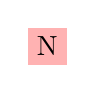
\begin{tikzpicture}
    \node [fill=red!30] {N};
  \end{tikzpicture}
  : \textit{lock} verrouillé\\
  \begin{tikzpicture}
    \node [label=left:$\to$] {N};
  \end{tikzpicture}
  : étape courante
\end{flushright}
\begin{center}
  \textit{Recherche du mot ``ln" dans le dictionnaire \{``nl", ``sln",
    ``su"\}}.
\end{center}


\subsection{Pruning}
On note:
\begin{itemize}
\item $t_a$ la taille du mot actuel
\item $t_r$ la taille du mot recherché
\item $d_a$ la distance du mot actuel au mot recherché
\item $d_m$ la meilleure distance trouvée jusqu'à présent entre un mot
  du dictionnaire et le mot recherché
\end{itemize}
On cherche à arrêter la recherche le plus tôt possible de trois
manières:
\begin{itemize}
\item Si $d_m = 1$, cela ne sert à rien de continuer car pour avoir une
  meilleure distance, il faudrait trouver le mot recherché dans le
  dictionnaire. Or la recherche par distance de Levenshtein est lancée
  uniquement si le mot n'existe pas tel quel dans le dictionnaire.

\textit{Exemple: Étape 2.}

\item La distance minimum entre deux mots est la différence de taille
  entre ces deux mots.
Si la taille du mot correspondant au n\oe{}ud actuel du Trie est supérieure
à la taille du mot recherché plus la meilleure distance trouvée
jusqu'à présent ($t_a > t_r + d_m$), alors on peut arrêter la
recherche sur cette branche.

\textit{Exemple: Étape 5.}

\item La distance entre le mot actuel et le mot recherché (la case en
  bas à droite du tableau) ne peut diminuer que de 1 lorsque l'on ajoute
  une ligne.
Donc il faut ajouter au minimum $d_a - d_m$ caractères pour avoir un
nouveau minimum.
Ce nouveau minimum potentiel aura un taille égale à $t_a + (d_a - d_m)$.
Si cette taille est supérieure à $t_r + d_m$, alors il n'y a aucune
chance pour que cette branche puisse trouver un nouveau minimum.
On peut donc s'arrêter.

\textit{Exemple: Étape 4.}
\end{itemize}

\subsection{Fine-grained locking}
26 branches partent de la racine du Trie.
Une opération peut travailler soit sur la racine, soit sur le reste de
l'arbre.
Si l'opération travaille sur la racine, un \textit{lock} global lui
assure l'exclusivité du dictionnaire.
Si l'opération ne travaille pas sur la racine (le cas le plus fréquent),
il travaille donc sur l'un des 26 fils de la racine.
Chacun de ces fils peut être \textit{lock} individuellement.
Si l'opération est une recherche, alors le compteur des \textit{readers}
pour cette branche est augmenté de 1.
Si l'opération modifie l'arbre, alors il attend qu'il n'y ait plus aucun
lecteur sur cette branche, puis il \textit{lock} la branche.

\section{AsyncDictionary}
Pour assurer la séquentialité du dictionnaire, nous avons utilisé un
système de ticket.
Il y a un compteur pour chaque type d'opération : \textit{search},
\textit{insert} et \textit{erase}.
Une opération d'un type ne peut pas s'exécuter si d'autres opérations
d'un autre type sont en cours d'exécution.
Par exemple, on ne peut pas faire un \textit{search} d'un mot avant
d'avoir exécuté toutes les insertions car cela pourrait changer le
résultat de la recherche.

Le thread désirant exécuter l'opération search incrémente le compteur de
search en attente mais ne commence pas tout de suite.
Il utilise un \texttt{std::condition\_variable} pour attendre que les
autres opérations soient finies.  Dès qu'il n'y a plus d'insertion ni de
suppression, toutes les recherches sont executées en même temps.

\end{document}
